%%%%%%%%%%%%%%%%%%%%%%%%%%%%%%%%%%%%%%%%%%%%%%%%%%%%%%%%%%%%%%%%%%%%%%%%%%%%%%%%%%%
%% Software Engineering: Project Management
%% CMMI: Project Monitoring and Control
%%
%% Tobias Stoll, Dominik Schreiber
%% winter term 2012/2013, TU Darmstadt
%%%%%%%%%%%%%%%%%%%%%%%%%%%%%%%%%%%%%%%%%%%%%%%%%%%%%%%%%%%%%%%%%%%%%%%%%%%%%%%%%%%
\documentclass[accentcolor=tud1b]{tudbeamer}

% ===== Packages ==================================================================
\usepackage[utf8]{inputenc}
\usepackage[ngerman]{babel}
\usepackage[T1]{fontenc}

\usepackage{color}
\usepackage{listings}
\usepackage{multicol}
\usepackage{eurosym}
\usepackage{amsmath}
%\usepackage[sectionbib]{natbib}
%\usepackage{chapterbib}

% ===== Commands, Changes =========================================================
\newcommand{\strong}[1]{\textaccentcolor{\textsf{\textbf{#1}}}}
\newcommand{\matheuro}{\text{\officialeuro}}

% ----- shorthand for creating a frame with current headline+subheadline ----------
\newcount\Level
\let\Part=\part\def\part{\global\Level=0\Part}
\let\Chapter=\chapter\def\chapter{\global\Level=1\Chapter}
\let\Section=\section\def\section{\global\Level=2\Section}
\let\Subsection=\subsection\def\subsection{\global\Level=3\Subsection}
\let\Subsubsection=\subsubsection\def\subsubsection{\global\Level=4\Subsubsection}

% creates a frame with a frametitle of up to two lines, depending on the current
% document structure. that means: 
% 	- if the tframe is created inside a section, it will have the sections header
% 	  as frametitle
% 	- if the tframe is created inside a subsection, it will have the sections
% 	  header as frametitle followed by the subsections header in the next line
% 	- if the tframe is created inside a subsubsection, it will have the subsections
% 	  header as frametitle followed by the subsubsections header in the next line
% each frametitle can be additionally adjusted by the optional argument. any text
% in there will be printed as \textnormal and appended to the second line with one
% space between the content and the appended text.
%
% usage:
% 	\begin{tframe}[optional addition to the subtitle]
% 		use it just as any normal frame
% 	\end{tframe}
\newenvironment*{tframe}[1][]{%
	\begin{frame}
	\ifnum\Level=2
		\frametitle{\insertsectionhead\\\strong{#1}}
	\fi\ifnum\Level=3
		\frametitle{\insertsectionhead\\\strong{\insertsubsectionhead} \textnormal{#1}}
	\fi\ifnum\Level=4
		\frametitle{\insertsubsectionhead\\\strong{\insertsubsubsectionhead} #1}
	\fi
}{%
	\end{frame}
}

% ===== Beamer Changes ============================================================
\AtBeginSection{
	\begin{frame}<beamer>{Outline}
		\tableofcontents[currentsection, currentsubsection, hideothersubsections]
	\end{frame}
}

% ===== Title =====================================================================
\title{CMMI: Project Monitoring and Control}
\author{Tobias Stoll, Dominik Schreiber}
\date{10.01.2013}

%%%%%%% Content %%%%%%%%%%%%%%%%%%%%%%%%%%%%%%%%%%%%%%%%%%%%%%%%%%%%%%%%%%%%%%%%%%%
\begin{document}

\begin{titleframe}
\end{titleframe}

% ===== Project Monitoring and Control ============================================
\section[Project Monitoring and Control]{The WHAT: Project Monitoring and Control, by Tobias Stoll}
\begin{tframe}

\cite{cmmi2010cmmidevelopment13}

\end{tframe}

% Maturity Level 2 (managed)
% short form: PMC
% purpose:
% - provide an understanding of the project's progress so that 
% - appropriate corrective actions can be taken when the 
% - project's performance deviates significantly from the plan.

\subsection{SG 1: Monitor the Project Against the Plan}
\begin{tframe}
	\begin{block}{Goal}
		\begin{itemize}
			\item identify \strong{actual} progress and performance against plan
			\item \strong{contrast} results with project plan
		\end{itemize}
	\end{block}
\end{tframe}

\subsubsection{SP 1.1: Monitor Project Planning Parameters}
\begin{tframe}
	\begin{itemize}
		\item measure \strong{actual} project planning parameters
		\item identify \strong{significant} deviations to the estimates in the plan
		\item record results
	\end{itemize}
	\begin{block}{SubPractices}
		\begin{itemize}
		  \item Monitor progress against schedule
		  \item Monitor the projects cost and expended effort
		  \item Monitor the attributes of the work products and tasks
		  \item Monitor resources provided and used
		  \item Monitor the knowledge and skills of the project personnel
		  \item Document the significant deviations in the project planning parameters
		\end{itemize}
	\end{block}
\end{tframe}

\subsubsection{SP 1.2: Monitor Commitments}
\begin{tframe}
	\begin{itemize}
		\item look at commitments
		\item compare them to identified commitments in the plan
	\end{itemize}
	\begin{block}{SubPractices}
		\begin{itemize}
		  \item Regularly review commitments
		  \item Identify commitments that have not been satisfied
		  \item Document the results of the commitment reviews
		\end{itemize}
	\end{block}
\end{tframe}

\subsubsection{SP 1.3: Monitor Project Risks}
\begin{tframe}
	\begin{itemize}
		\item Monitor risks against those in the plan
	\end{itemize}
	\begin{block}{SubPractices}
		\begin{itemize}
		  \item Periodically review the documentation of the risks
		  \item Revise the documentation of the risks
		  \item Communicate risk status to relevant stakeholders
		\end{itemize}
	\end{block}
\end{tframe}

\subsubsection{SP 1.4: Monitor Data Management}
\begin{tframe}
	\begin{itemize}
		\item check data management activities
		\item ensure compliance of data management plans
	\end{itemize}
		\begin{block}{SubPractices}
		\begin{itemize}
		  \item Periodically review data management activities
		  \item Identify and document significant issues and their impacts
		  \item Document the results of data management activity reviews
		\end{itemize}
	\end{block}
\end{tframe}

\subsubsection{SP 1.5: Monitor Stakeholder Involvement}
\begin{tframe}
	\begin{itemize}
		\item detect involvement of identified stakeholders 
		\item ensure that the right interactions occure
	\end{itemize}
	\begin{block}{SubPractices}
		\begin{itemize}
		  \item Periodically review the status of stakeholder involvement
		  \item Identify and document significant issues and their impacts
		  \item Document the results of the stakeholder involvement status reviews
		\end{itemize}
	\end{block}
\end{tframe}

\subsubsection{SP 1.6: Conduct Progress Reviews}
\begin{tframe}
	\begin{itemize}
		\item project reviews to inform stakeholders
		\item may not be specified in project plan
	\end{itemize}
	\begin{block}{SubPractices}
		\begin{itemize}
		  \item Regularly communicate status on assigned activities and work products to relevant stakeholders
		  \item Review the results of collecting and analyzing measures for controlling the project
		  \item Identify and document significant issues and deviations from the plan
		  \item Document change requests and problems identified in any of the work products and processes
		  \item Document the results of the reviews
		  \item Track change requests and problem reports to closure
		\end{itemize}
	\end{block}
\end{tframe}

\subsubsection{SP 1.7: Conduct Milestone Reviews}
\begin{tframe}
	\begin{itemize}
		\item review of results at selected milestones
		\item typically formal and planned 
	\end{itemize}
	\begin{block}{SubPractices}
		\begin{itemize}
		  \item Conduct reviews at meaningful points in the projects schedule
		  \item Review the commitments, plan, status, and risks of the project
		  \item Identify and document significant issues and their impacts
		  \item Document the results of the review, action items, and decisions
		  \item Track action items to closure
		\end{itemize}
	\end{block}
\end{tframe}

\subsection{SG 2: Manage Corrective Action to Closure}
\begin{tframe}
	\begin{block}{Goal}
		\begin{itemize}
		  	\item react with significant deviations from plan
			\item take corrective actions
		\end{itemize}
	\end{block}
\end{tframe}

\subsubsection{SP 2.1: Analyze Issues}
\begin{tframe}
	\begin{itemize}
		\item 
	\end{itemize}
	\begin{block}{SubPractices}
		\begin{itemize}
		  \item Gather issues for analysis
		  \item Analyze issues to determine need for corrective action
		\end{itemize}
	\end{block}
\end{tframe}

\subsubsection{SP 2.2: Take Corrective Action}
\begin{tframe}
	\begin{itemize}
		\item 
	\end{itemize}
	\begin{block}{SubPractices}
		\begin{itemize}
		  \item Determine and document the appropriate actions needed to address the identified issues
		  \item Review and get agreement with relevant stakeholders on the actions to be taken
		  \item Negotiate changes to internal and external commitments
		\end{itemize}
	\end{block}
\end{tframe}

\subsubsection{SP 2.3: Manage Corrective Actions}
\begin{tframe}
	\begin{itemize}
		\item 
	\end{itemize}
	\begin{block}{SubPractices}
		\begin{itemize}
		  \item Monitor corrective actions for completion
		  \item Analyze results of corrective actions to determine the effectiveness
		  \item Determine and document appropriate actions to correct deviations
		\end{itemize}
	\end{block}
\end{tframe}

% ===== industrial practices =======================================================
\section[industrial practices]{The HOW (part 1): industrial practices, by Dominik Schreiber}
\begin{tframe}
	
\cite{alegria2006cmmiagile}

\end{tframe}

% ----- scrum ----------------------------------------------------------------------
\subsection{Scrum}
\begin{tframe}[- what it is]
	\begin{multicols}{2}
		\begin{block}{Overview}
			\begin{itemize}
				\item \strong{agile} software-engineering process
				\item \strong{iterative}: thinking in \emph{sprints}
				\item \strong{slim}: 3 \emph{roles}, 4 \emph{artifacts}, small set of \emph{rules}
				\item \strong{communicative}: daily meetings, planning, reviews (but less paperwork)
			\end{itemize}
		\end{block}
		\begin{figure}
			\centering
			\includegraphics[width=.45\textwidth]{img/scrum-process.png}
			\caption{scrum process overview}
		\end{figure}
	\end{multicols}
\end{tframe}

\begin{tframe}[- how it supports PMC]
	\begin{block}{Regular meetings}
		\begin{itemize}
			\item \strong{Sprint planning meeting} (part 1: whole team): 
				\begin{itemize}
					\item clean product backlog, prioritize entries
					\item choose entries for next sprint
				\end{itemize}
			\item \strong{Sprint planning meeting} (part 2: developers):
				\begin{itemize}
					\item convert entries to 1-day tasks ($\Rightarrow$ sprint backlog)
					\item extract sprint-goal from entries
				\end{itemize}
			\item \strong{Sprint Review}:
				\begin{itemize}
					\item present product to product owner, check sprint-goal
					\item give feedback for last sprint, update product backlog
				\end{itemize}
			\item \strong{Sprint Retrospective}:
				\begin{itemize}
					\item concrete improvements based on
					\item feedback for the last sprint
				\end{itemize}
		\end{itemize}
	\end{block}
\end{tframe}

\begin{tframe}[]
	\begin{multicols}{2}
		\begin{figure}
			\centering
			\includegraphics[width=.45\textwidth]{img/Scrum-taskboard.jpg}
			\caption{Scrum Taskboard}
		\end{figure}
		\begin{figure}
			\centering
			\includegraphics[width=.45\textwidth]{img/Scrum-burndown-chart.jpg}
			\caption{Scrum Burndown Chart}
		\end{figure}
	\end{multicols}
\end{tframe}

% ----- extreme programming ---------------------------------------------------------
\subsection{Extreme Programming}
\begin{tframe}[- what it is]
	\begin{block}{Overview}
		\begin{itemize}
			\item \strong{agile} software-engineering process
			\item strong \strong{principles}: Pair Programming, Test-driven Development, Continuous Integration, \dots
		\end{itemize}
	\end{block}
	\pause
	\begin{block}{Differences to Scrum}
		\begin{itemize}
			\item \strong{iteration length}: week (XP) $\leftrightarrow$ month (Scrum)
			\item \strong{change adaption}: always (XP) $\leftrightarrow$ not in current sprint (Scrum)
			\item \strong{work order}: customer chooses (XP) $\leftrightarrow$ team chooses (Scrum)
			\item \strong{engineering practices}: given (XP) $\leftrightarrow$ not given (Scrum)
		\end{itemize}
	\end{block}
\end{tframe}

\begin{tframe}[- how it supports PMC]
	\begin{block}{through the engineering process}
		\begin{itemize}
			\item \strong{Planning Game}: release+iteration planning match results with plan constantly, split up in 3 phases:
			\begin{multicols}{3}
				\begin{enumerate}
					\item \emph{exploration phase}\\{\scriptsize create user stories/split them into tasks}
					\item \emph{commitment phase}\\{\scriptsize commit to func\-tion\-ali\-ties/assign tasks}
					\item \emph{steering phase}\\{\scriptsize adjust plan/perform tasks, match result to plan}
				\end{enumerate}
			\end{multicols}
			\item \strong{Test-driven Development}: all productive code is written to make failing unit tests pass $\rightarrow$ unit tests describe the plan
			\item \strong{Continuous Integration}: automated unit tests match every commit to the plan
		\end{itemize}
		it is the \strong{combination} of the 12 principles that makes XP work
	\end{block}
\end{tframe}

% ----- representations of progress -------------------------------------------------
\subsection{methodology-independent representations of progress}
\begin{tframe}
	\begin{multicols}{2}
		\begin{block}{gantt chart}
			\begin{itemize}
				\item illustrates project \strong{schedule}
				\item project is broken down into elements
				\item each element has \strong{start} and \strong{end}
				\item progress of each element can be illustrated
			\end{itemize}
		\end{block}
		\begin{block}{network diagram}
			\begin{itemize}
				\item shows \strong{dependencies} in schedule
				\item same information as gantt chart, different representation
			\end{itemize}
		\end{block}
		\begin{figure}
			\centering
			\includegraphics[width=.35\textwidth]{img/gantt-chart.png}\\\vspace{.3cm}
			\includegraphics[width=.45\textwidth]{img/network-diagram.png}
			\caption{gantt chart, network diagram}
		\end{figure}
	\end{multicols}
\end{tframe}

% ----- earned-value analysis ------------------------------------------------------
\subsection{Earned-Value Analysis}
\begin{tframe}[- what it is]
	\begin{multicols}{2}
		\begin{figure}
			\centering
			\includegraphics[width=.45\textwidth]{img/earned-value-analysis.png}
			\caption{combined values in EVA}
		\end{figure}
		\begin{block}{project controlling tool}
			\begin{itemize}
				\item allows \strong{monitoring} of \emph{scope}, \emph{schedule} and \emph{cost} of a project
				\item allows \strong{forecasts} for the evolving project
				\item not restricted to software engineering, works for \strong{all kinds of projects}
			\end{itemize}
		\end{block}
	\end{multicols}
\end{tframe}

\begin{tframe}[- how it works]
	\begin{multicols}{2}
		\begin{block}{measured values}
			\begin{itemize}
				\item \strong{planned cost} (\emph{PC}): pre-defined cost for the \emph{whole project}
				\item \strong{actual cost} (\emph{AC)}: actual cost \emph{until now}
			\end{itemize}
		\end{block}
		\begin{block}{metrics}
			\begin{itemize}
				\item \strong{earned value} (\emph{EV}): actual \emph{value} of the work until now\\{\scriptsize simple metric: $EV = Budget \cdot \%Progress$}
			\end{itemize}
		\end{block}
		\begin{block}{derived values}
			\begin{itemize}
				\item \strong{schedule variance}:\\$SV = EV - PC$
				\item \strong{cost variance}:\\$CV = EV - AC$
				\item \strong{schedule performance index}:\\$SPI = \frac{EV}{PC}$
				\item \strong{cost performance index}:\\$CPI = \frac{EV}{AC}$
			\end{itemize}
		\end{block}
	\end{multicols}
\end{tframe}

\begin{tframe}[- example]
	\begin{multicols}{2}
		\begin{block}{your task}
			\begin{itemize}
				\item list of \strong{500} hand-written mail addresses
				\item insert this into \strong{mailing list}
				\item you need \strong{2h} for this, get \strong{10\euro{/h}}
				\item \strong{half time!} 1h left
			\end{itemize}
		\end{block}
		\begin{block}{measured values}
			\begin{itemize}
				\item \strong{PC} = $20\matheuro \cdot \frac{1}{2} = 10\matheuro$
				\item \strong{AC} = $10\frac{\matheuro}{1h} \cdot 1h = 10\matheuro$
			\end{itemize}
		\end{block}
		\begin{block}{metrics}
			\begin{itemize}
				\item you were \strong{fast}! Did 300 already!
				\item \strong{EV} = $20\matheuro \cdot \frac{300}{500} = 12\matheuro$
			\end{itemize}
		\end{block}
		\begin{block}{derived values}
			\begin{itemize}
				\item \strong{SV} = $12\matheuro - 10\matheuro = 2\matheuro$
				\item \strong{CV} = $12\matheuro - 10\matheuro = 2\matheuro$
				\item \strong{SPI} = $\frac{12\matheuro}{10\matheuro} = 1.2$
				\item \strong{CPI} = $\frac{12\matheuro}{10\matheuro} = 1.2$
			\end{itemize}
		\end{block}
	\end{multicols}
	\pause
	If you stay that fast, you'll finish \strong{20min early}. Means: you'll get \strong{\euro{3,30}} for free.
\end{tframe}

% ===== real-life examples =========================================================
\section[real-life examples]{The HOW (part 2): real-life examples, by Dominik Schreiber}

% ----- openlearnware --------------------------------------------------------------
\subsection{at openLearnWare}
\begin{tframe}[- project overview]
	\begin{multicols}{2}
		\begin{block}{Project: material portal for students}
			\begin{itemize}
				\item webservice for lecture material
				\item development started in spring 2010
				\item team of 2 full-time employees, 5 HiWis
				\item scrum-like project structure
			\end{itemize}
		\end{block}
		\begin{figure}
			\centering
			\includegraphics[width=.45\textwidth]{img/olw-screenshot.png}
			\caption{\href{http://www.tu-darmstadt.de/olw}{tu-darmstadt.de/olw}, 7.1.13}
		\end{figure}
	\end{multicols}
\end{tframe}

\begin{tframe}[- project structure]
	\begin{multicols}{2}
		\begin{figure}
			\centering
			\includegraphics[width=.45\textwidth, draft]{img/olw-taskboard.png} % TODO remove draft
			\caption{taskboard, december-sprint}
		\end{figure}
		\begin{block}{team members}
			\begin{itemize}
				\item ``Intellectual head'' -- like Scrum's \strong{product owner}, responsible for all ``non-technical stuff''
				\item ``Technical head'' -- like Scrum's \strong{scrum master}, responsible for all ``technical stuff''
				\item 5 HiWis, working 8-20 hours a week -- the \strong{scrum team}
			\end{itemize}
		\end{block}
	\end{multicols}
\end{tframe}

\begin{tframe}[- project monitoring/control]
	\begin{multicols}{2}
		\begin{block}{process items}
			\begin{itemize}
				\item weekly \strong{scrum meeting} -- about an hour, with all team members
				\item weekly \strong{planning meeting} -- about 2 hours, intellectual+technical head
				\item \strong{taskboard} as a mirror of the redmine \emph{ticket system}
				\item \strong{tickets} as a \emph{sprint backlog}
				\item current \strong{QSL-Request} as \emph{product backlog}
				\item \strong{Jenkins} as \emph{Continuous-Integration Server}
			\end{itemize}
		\end{block}
		\begin{figure}
			\centering
			\includegraphics[width=.35\textwidth]{img/olw-redmine.png}\\
			\includegraphics[width=.35\textwidth]{img/olw-jenkins.png}
			\caption{ticket system, ci-server}
		\end{figure}
	\end{multicols}
\end{tframe}

\begin{tframe}[- how the process evolved]
	\begin{multicols}{2}
		\begin{figure}
			\centering
			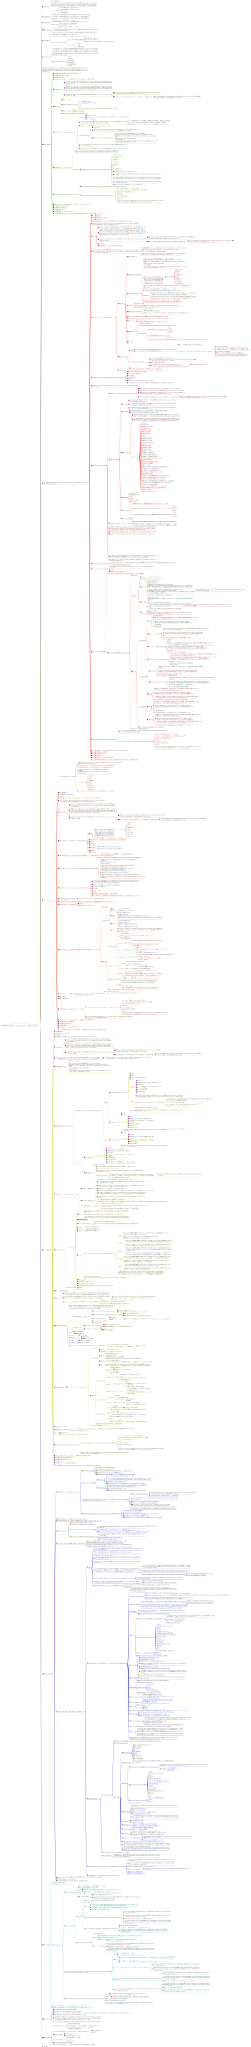
\includegraphics[height=.85\textheight]{img/olw-mindmap.pdf}
			%\includegraphics[height=.85\textheight]{img/olw-mindmap-expanded.png}	
			\caption{former product backlog}
		\end{figure}
		\begin{block}{change as the only constant}
			\begin{itemize}
				\item no current team member from the \strong{founder team}
				\item began with \strong{giant mind-maps} as product/sprint backlogs
				\item had 2-3 nearly \strong{complete restarts}
				\item in the beginning: \strong{no documentation} at all (except backlogs)
			\end{itemize}
		\end{block}
	\end{multicols}
\end{tframe}

% ----- dimetis GmbH ---------------------------------------------------------------
\subsection{at dimetis GmbH}
\begin{tframe}

\end{tframe}

% ----- major-client software-engineering company ----------------------------------
\subsection{at a major-client software-engineering company}
\begin{tframe}
	\begin{block}{Project: Web-based software for the government}
		\begin{itemize}
			\item up to 1.5 years \strong{specification phase}
			\item teams of \strong{<10 members}
			\item project head spends \strong{1 day a week} with the customer
		\end{itemize}
	\end{block}
\end{tframe}

\begin{tframe}
	\begin{block}{the process}
		\begin{itemize}
			\item \strong{specification phase}: before the project starts, it gets strongly \emph{specified} (customer reviews this)
			\item \strong{implementation}: according to system specification, features are implemented
			\item \strong{internal reviews}: code is reviewed twice: once technical, once specialist
			\item \strong{small releases}: working features are shipped to the customer early, loaded with unit tests/performance tests/specific tests
			\item \strong{issue tracking}: customer show occuring bugs to developers or reports them in the issue tracker
		\end{itemize}
	\end{block}
\end{tframe}

% ===== post-presentation ==========================================================
\begin{frame}{Thank you for your attention!}
\begin{center}
\pause
\vspace{1cm}

I want to hear at least \strong{3 questions} from you.
\vspace{1cm}

\noindent{\huge Start now!}
\end{center}
\end{frame}

% ===== appendix: bibliography =====================================================
\appendix
\begin{frame}{Bibliography}
	\bibliographystyle{alphanum}
	\bibliography{cmmi-monitoring}
\end{frame}

% ===== backup slides ==============================================================
\begin{frame}{Extreme Programming\\\strong{Principles}}
\label{fr:xp-principles}
	\begin{multicols}{2}
		\begin{block}{Fine scale feedback}
			\begin{itemize}
				\item pair programming
				\item planning game
				\item test-driven development
				\item whole team
			\end{itemize}
		\end{block}
		\begin{block}{continuous process}
			\begin{itemize}
				\item continuous integration
				\item refactoring/design improvement
				\item small releases
			\end{itemize}
		\end{block}
		\begin{block}{shared understanding}
			\begin{itemize}
				\item coding standards
				\item collective code ownership
				\item simple design
				\item system metaphor
			\end{itemize}
		\end{block}
		\begin{block}{programmer welfare}
			\begin{itemize}
				\item sustainable pace
			\end{itemize}
			\vspace{1cm}
		\end{block}
	\end{multicols}	
\end{frame}

\end{document}